	\documentclass[14pt]{extreport}
\usepackage{extsizes}
	\usepackage[frenchb]{babel}
	\usepackage[utf8]{inputenc}  
	\usepackage[T1]{fontenc}
	\usepackage{amssymb}
	\usepackage[mathscr]{euscript}
	\usepackage{stmaryrd}
	\usepackage{amsmath}
	\usepackage{tikz}
\usepackage{eurosym}
	\usepackage[all,cmtip]{xy}
	\usepackage{amsthm}
	\usepackage{varioref}
	\usetikzlibrary{patterns}
	\usepackage{float}
	\usepackage[ margin=1in]{geometry}
	\geometry{a4paper}
	\usepackage{lmodern}
	\usepackage{hyperref}
	\usepackage{array}
	\usepackage{easytable}
	 \usepackage{fancyhdr}\usepackage{longtable}

	\pagestyle{fancy}
	\theoremstyle{plain}
	\fancyfoot[C]{\empty} 
	\fancyhead[L]{Contrôle}
	\fancyhead[R]{21 mai 2024}
	
	
	\title{Contrôle chapitre 6}
	\date{}
	\begin{document}

\begin{center}{\Large Contrôle chapitre 8}\\ \textbf{Soignez votre présentation et votre rédaction.}\end{center}

\textbf{Exercice 1}  % 4 points

Donner le périmètre et l'aire contenue à l'intérieur des figures suivantes : \begin{itemize}
\item Un carré dont un côté mesure $2$ cm. 
\item Un rectangle de longueur $3,2$ dm et de largeur $3,7$ dm. 
\item Un cercle de rayon $4$ cm (donner la valeur exacte, puis une valeur approchée au mm).
\item Le triangle ci-dessous. 
\begin{figure}[H]\center
\begin{tikzpicture}[scale = 3]
\draw (-0.5, 0) --  (3.5, 0) -- (0, 1.2) -- (-0.5, 0);
\draw[dashed] (0,0) -- (0,1.2); 
\draw [<->] (-0.5, -.1) -- (0, -.1); 
\draw [<->] (3.5, -.1) -- (0, -.1); 
\draw (-.25, -.2) node {$1,5$ cm};
\draw (1.65, -.2) node {$10,5$ cm};
%\draw [<->] (0.05, 0) -- (0.05, 1.2); 
\draw (0.29, .6) node {$3,6$ cm};
\draw (1.6, .8) node {$11,1$ cm};
\draw (-0.6, .6) node {$3,9$ cm};
\fill (0.1,0) -- (0.1, 0.1) -- (0, 0.1) -- (0,0);
\end{tikzpicture}
\end{figure}
\end{itemize}

\ 

\textbf{Exercice 2}

On considère un champ dont le tracé est le suivant : 
\[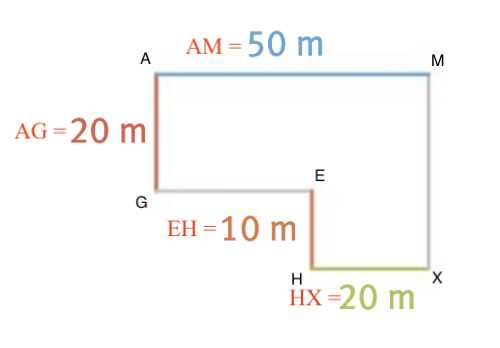
\includegraphics[scale=.75]{Exo3.png}\]

1) Calculer la longueur de la clôture nécessaire pour entourer ce champ. 

2) Calculer la surface du champ. 

3) On doit répandre de l'engrais sur le champ, à raison de $2$ litres par mètre carré. Quelle quantité va-t-on utiliser ? 

\newpage

\textbf{Exercice 3}
On considère les deux figures suivantes : 

\begin{figure}[H]
\center 
\begin{tikzpicture}[scale =1.3]
\draw (-2, 0) -- (2, 0) arc (0: 180 :2);
\fill[pattern=north west lines] (-2, 0) -- (2, 0) arc (0: 180 :2);
\draw[<->] (-2, -.1) -- (2, -.1); 
\draw (0, -.5) node {$4\ cm$};
\draw[white](0,-1)--(3,-1);
\end{tikzpicture}
\begin{tikzpicture}[scale =1.3]
\draw[dashed](-2, 0) -- (2, 0);
\draw(2,0) arc (0: 180 :2) arc (180:360: 1) arc(180:0:1);
\fill[pattern=north west lines](2,0) arc (0: 180 :2) arc (180:360: 1) arc(180:0:1);
\draw[<->] (2, -.1) -- (0, -.1); 
\draw (1, -.5) node {$2\ cm$};
\end{tikzpicture}
\end{figure} 

1) Calculer le périmètre des deux figures. Donner d'abord la valeur exacte, puis la valeur approchée au millimètre. 

2) Calculer les aires des deux figures. Donner d'abord la valeur exacte, puis la valeur approchée au millimètre carré. 

\textbf{Exercice 4}


On considère la figure suivante, où $AC = 4$ cm et $BD = 2$ cm. 

\begin{figure}[H]
\center 
\begin{tikzpicture}[scale =1.3]
\draw (-2,0) -- (0,1) -- (2,0) -- (0,-1) -- (-2,0) ; 
\draw (-2,0) -- (0,1) -- (2,0) -- (0,-1) -- (-2,0) ; 
\draw[dashed] (-2,0) -- (2,0) (0,-1) -- (0,1);
\draw (-2.2, 0) node{A} (0,1.2) node{B} (2.2,0) node{C} (0,-1.2) node{D};
\draw (-1, .5) circle (.1) (1, .5) circle (.1) (1, -.5) circle (.1) (-1, -.5) circle (.1);
\draw (0.2, 0.2) node{O}; 
\end{tikzpicture}
\end{figure} 

1) Le quadrilatère $ABCD$ est un losange. Rappeler la définition d'un losange. 

2) Que dire des diagonales d'un losange ? 

3) En déduire que le triangle $AOB$ est rectangle en $O$. 

4) Calculer l'aire du triangle $AOB$. 

5) En déduire l'aire du losange $ABCD$. 
 


\end{document}